%Inizio Preambolo

% Prepara un documento per carta A4, con un bel font grande
\documentclass[a4paper,12pt]{book}
\usepackage[italian]{babel} % Consente l'uso caratteri accentati italiani
\usepackage[utf8]{inputenc}
\usepackage{fullpage}
\usepackage{color} 
\definecolor{grayback}{rgb}{0.9,0.9,0.9}
\definecolor{grayrows}{rgb}{0.5,0.5,0.5} 
\usepackage{graphicx}
\usepackage{listings} 


\graphicspath{img/}

\frenchspacing % forza LaTeX ad una spaziatura fra parole non inglese

\title{Relazione del Progetto di Linguaggi e Compilatori} 
\author{Luca Cividini, Fabio Marini, Antonio Riva}
\date{giugno 2007}

\lstdefinestyle{num_righe}{
	numbers=left,
    stepnumber=1,
    numberstyle=\footnotesize\color{grayrows},
    numbersep=10pt,
    firstnumber=1
}

\lstdefinelanguage{model}{
morekeywords={class,package,relations,attributes,methods,public,private,protected,use,extend,depend,associate,include,composed,realize}
,morestring=[b]",
    morecomment=[l]{//},    morecomment=[l]{\#},
    morecomment=[s]{/*}{*/}
}

\lstdefinelanguage{layout}{
morekeywords={import,class,\@margin,\@hide-args,\@collapse,\@layout}
	,morestring=[b]",
    morecomment=[l]{//},    morecomment=[l]{\#},
    morecomment=[s]{/*}{*/}
}


\lstdefinestyle{none}{
	frame=ltrb,
	tabsize=2,
	basicstyle=\small,
	keywordstyle={\color{blue}\bfseries},
	identifierstyle=\ttfamily,
	stringstyle=\ttfamily,
	captionpos=t,
	abovecaptionskip=15pt,
	showstringspaces=false,
	style=num_righe,
	commentstyle={\color{grayrows}\bfseries},
    morecomment=[l]{//},    morecomment=[l]{\#},
    morecomment=[s]{/*}{*/}
}

\lstdefinestyle{model}{
	language=model,
	style=none
}

\lstdefinestyle{java}{
	language=java,
	style=none
}

\lstdefinestyle{layout}{
	language=layout,
	style=none
}
%Fine Preambolo

\begin{document}
\maketitle % Produce effettivamente il titolo a partire dai comandi \title,\author e \date

\tableofcontents % Prepara l'indice generale
%\input{include/bibliography.bib}

\chapter{Introduzione}

Per l'esame di ``\emph{progetto di linguaggi e compilatori}'' abbiamo deciso di
basarci sul progettino consegnato per l'esame ``\emph{linguaggi e compilatori}''
tenuto lo scorso semestre. \\*
L'obiettivo di tale progettino è stata la definizione del linguaggio per la 
descrizione di diagrammi UML. In particolar modo si era prestata attenzione al
controllo di dichiarazione/uso/non redichiarazione
delle classi e a controlli di non re-dichiarazione di package.




\section{cUml2Svg - Coded UML to SVG} 
Il progetto da noi sviluppato si chiama \emph{cUml2Svg}. \\*
L'acronimo \emph{cUml2Svg} sta per ``\emph{Coded UML to SVG}"; 
il progetto consiste nello sviluppare un traduttore che traduca da una
rappresentazione in codice dei digrammi UML delle classi alla rappresentazione
grafica tipica dell'UML.\\*
La rappresentazione grafica da noi scelta e sulla quale abbiamo basato il nostro
progetto è l'SVG.\\*
L'SVG (Scalable Vector Graphics), indica una tecnologia in grado di visualizzare oggetti 
di grafica vettoriale e, pertanto, di gestire immagini scalabili dimensionalmente.
Più specificamente si tratta di un linguaggio derivato dall'XML, che si pone l'obiettivo 
di descrivere figure bidimensionali statiche o animate. \\*
In Particolare SVG permette di trattare tre tipi di oggetti grafici:

\begin{itemize}
  \item forme geometriche, cioè linee costituite da segmenti di retta, curve e
  aree delimitate da linee chiuse;
  \item immagini della grafica raster e immagini digitali;
  \item testi esplicativi, eventualmente cliccabili.
\end{itemize} 


Per utilizzare al meglio il nostro progetto abbiamo sviluppato anche una 
interfaccia grafica, che aiuta nella stesura dei modelli e degli schemi da
utilizzare. in particolare abbiamo sviluppato il text-highlight, i
controlli degli errori (errori di sintassi, errori semantici e warning) e la
compilazione automatica.
L'interfaccia grafica è stata costruita
come estensione del popolare ambiente di sviluppo Eclipse~\cite{eclipse_website:1}

%luca
\chapter{Il linguaggio}

Il linguaggio che stiamo proponendo è strutturato in 2 parti, e quindi due tipi di
file, che corrispondono al concetto di modello e layout; non a caso l'estensione
del primo è u2sm e il secondo è u2sl.

Il file modello sarà il contenitore delle definizione delle classi mentre nel
file layout il programmatore indicherà l'aspetto grafico del diagramma che si va
a generare.

\section{Model}

Il modello (estensione .u2sm) conterrà quindi tutte le informazioni riguardo il
contenuto/i dati
degli elementi che sarà possibile inserire in un diagramma in un secondo
momento. 

In un linguaggio ad oggetti uno degli strumenti fondamentali è la suddivisione 
delle classi sotto forma di package. Nella nostra proposta un file di modello
può contenere o una lista di classi (non associate ad un package) oppure una
lista di package.

La definizione del package (come un po' tutto il nostro linguaggio) è 
ispirata alla sintassi dei linguaggi java like.

\begin{lstlisting}[caption={Dichiarazione di package}, style={model}]
package nome.pkg{
	...  	
}
\end{lstlisting}

Nella definizione della classe è invece dichiarato in modo esplicito la
suddivisione tra i componenti base di una classe; sono quindi esplicitati quali
sono gli attributi, i metodi e le relazioni. L'aggiunta delle relazioni rispetto
ad una classica definizione di classe è necessaria per poter rappresentare nel
diagramma le frecce di collegamento.


\begin{lstlisting}[caption={Dichiarazione di classe}, style={model}]
class NomeClasse{
	relations{
		...
	}
	attributes{
		...
	}
	methods{
		...
	}
}
\end{lstlisting}

E' anche possibile dichiarare delle Interfacce utilizzando la parola chiave
interface al posto di class. 

\begin{figure}[htp]
\begin{center}
  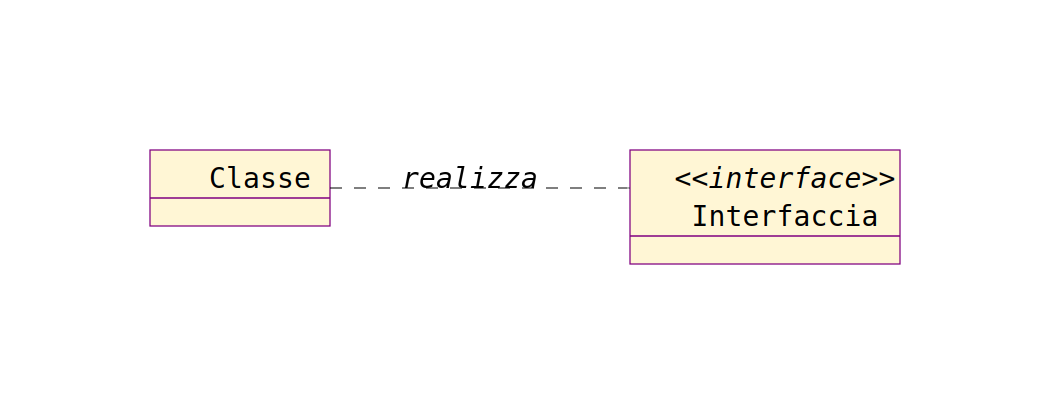
\includegraphics[width=0.8\textwidth]{img/class_interface}
  \caption[labelInTOC]{La visualizzazione di una classe vuota e di
  un'interfaccia vuota}
\end{center}
\end{figure}


Analizziamo ora il contenuto delle varie sezioni.

\subsection{Relazioni}

Nella sezione delle relazioni
viene appunto dichiarata una lista di definizione che contiene il tipo della 
relazione, una lista di classi (complete di package) 
con cui creare una relazione del tipo scelto
per ogni classe 3 parametri opzionali (che possono anche essere vuoti) in cui
il primo parametro e l'ultimo possono essere utilizzati per la definizione delle
cardinalità, mentre il parametro opzionale può essere utilizzato per definire
una descrizione della relazione; queste stringhe andranno a posizionarsi sul 
disegno delle frecce.

\begin{lstlisting}[caption={Dichiarazione di relazione}, style={model}]
relations{
	extend nome.pkg.NomeClasse ("(1,*)" , 
				"descrizione relazione", "(1,1)" );
	use nome.pkg.NomeClasse1, nome.pkg.NomeClasse2;
}
\end{lstlisting}

La lista dei possibili tipi di relzione sono:
\begin{itemize}
  \item{use (uso);}
  \item{extend (ereditarietà);}
  \item{associate (associazione);}
  \item{include (inclusione);}
  \item{realize (realizzazione);}
  \item{depend (dipendenza);}
  \item{composed (composizione);}
\end{itemize}

Di seguito un digramma creato per visualizzare tutti i tipi di relazione.

\begin{figure}[htp]
\begin{center}
  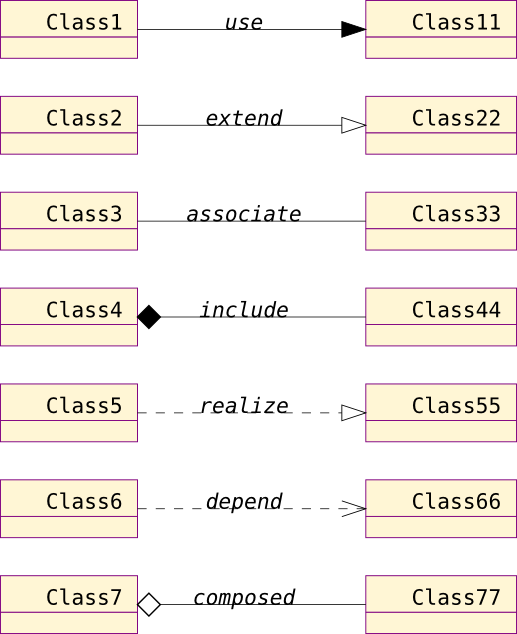
\includegraphics[width=0.5\textwidth]{img/relation_arrow}
  \caption[labelInTOC]{I vari tipi di relazione}
\end{center}
\end{figure}


\subsection{Attributi}

Gli attributi vengono dichiarati come visibilità:
\begin{itemize}
  \item public
  \item private
  \item protected
\end{itemize}

tipo (opzionale), nome attributo e valore di default (opzionale); la sintassi è
quella indicata nell'esempio sottostante.

\begin{lstlisting}[caption={Dichiarazione di attributi}, style={model}]
attributes{
	public int attr1=5;
	public "ArrayList<Integer>" attr2;
	private attr3;
}
\end{lstlisting}

Un ulteriore osservazione che si può fare è che i tipi (anche per i metodi e gli 
argomenti dei metodi) possono essere indicati come stringhe in modo da poter 
rappresentare situazioni con tipi contenenti caratteri speciali, come per esempio
un tipo ``generico''.

\subsection{Metodi}

Anche in questo caso la definizione dei metodi è del tutto simile alla
definizione della segnatura di un metodo in java.

\begin{lstlisting}[caption={Dichiarazione di metodi}, style={model}]
methods{
	public nomeMetodo1(int arg1=10, String arg2,arg3);
	private nomeMetodo2(arg1);
	nomeMetodo3();
}
\end{lstlisting}

Nell'esempio di definizione sopra riportato si possono contraddistinguere varie 
caratteristiche aggiuntive del nostro linguaggio; un metodo è caratterizzato
oltre che dal suo nome anche dal tipo di visibilità.

Gli attributi possono essere definiti sia con l'assegnazione di un tipo che con
la definizione del solo nome, c'è anche la possibilità di assegnare un valore di
default al parametro del metodo (caratteristica disponibile in alcuni linguaggi
tipo il PHP).
Possiamo notare il fatto che è possibile omettere gran parte degli attributi
perché l'idea è che deve essere obbligatorio definire solo gli elementi minimi
per poi poter indicare, opzionalmente, solo ciò che si vuole rappresentare nel
diagramma. 


\section{Layout}


Una volta specificato il modello si procede con il disegnare il diagramma
attraverso la definizione di un file di layout (estensione .u2sl).

Come prima cose bisogna associare al layout i modelli da utilizzare questa
operazione si effettua con il comando import; si possono importare più file
modello, ma devono essere importati come prime righe,altrimenti il compilatore
non sa cosa disegnare. E' possibile che ci sia il caso in cui la stessa classe è
contenuta in più file modello, la regola è che il primo dichiarato rimane; verrà
comunque segnalato un errore. Il percorso del file è un percorso relativo
rispetto al path in cui è salvato il file layout.

\begin{lstlisting}[caption={Import dei modelli necessari}, style={layout}] 
import test.u2sm;
\end{lstlisting}

La logica di definizione del modello si basa sul concetto delle scatole cinesi (o
dei gruppi); un gruppo viene definito attraverso l'uso delle parentesi quadre,
un gruppo può contenere altri gruppi o una definizione di classe.

Il codice sottostante definisce 2 gruppi; il primo contenente 2 sottogruppi e
 con una dichiarazione di classe per ogni gruppo di livello più basso.

\begin{lstlisting}[caption={Un semplice diagramma}, style={layout}] 
[
	[
		(class nome.pkg.NomeClasse1)
	]
	[
		(class nome.pkg.NomeClasse2)
	]
]
[
	(class nome.pkg.NomeClasse3)
]
\end{lstlisting}

In questo modo è molto semplice definire dei gruppi di oggetti da legare tra di
loro. Per ogni gruppo è possibile specificare delle proprietà subito dopo
l'apertura della parentesi che modificano l'aspetto del gruppo o delle classi in
esso contenute; le proprietà disponibili sono:

\begin{itemize}
  \item @layout i cui calori possono essere:
  \begin{itemize}
  	\item Nx* dove N è il numero di righe su cui disporre le classi;
  	\item *xN dove N è il numero di colonne su cui disporre le classi;
  	\item *x* per disporre le classi in un quadrato di lato uguale alla radice
  	quadrata del numero di elementi del gruppo;
  \end{itemize}
  
  \item @margin con quattro numeri che indicano il margine superiore (top),
  destro (right), inferiore (bottom), sinistro (left);
  \item @collapse che prende come parametri all, methods, attributes; per far in
  modo di non visualizzare i metodi o gli attributi o tutti e due;
  \item @hide-args che permette di nascondere gli argomenti dei metodi.
\end{itemize}

\begin{lstlisting}[caption={Diagramma decorato di attributi}, style={layout}] 
[
	[	
		@margin 15 10 5 0
		@collapse all
		(class nome.pkg.NomeClasse1)
	]
	[
		@collapse methods
		@hide-args
		(class nome.pkg.NomeClasse2)
	]
]
[
	@layout *x1
	@collapse attributes
	(class nome.pkg.NomeClasse3)
	(class nome.pkg.NomeClasse4)
]
\end{lstlisting}


Come è possibile notare dagli esempi di codice superiori l'introduzione di una
classe nel diagramma è dettata dal nome della classe circondato da parentesi
tonde all'interno di un gruppo.

Il nome della classe può essere indicato per esplicito inserendo il nome della
classe comprensivo di package oppure si possono inserire tutte le classi di un
package semplicemente indicando il package e facendolo seguire da un ``.*''.

Un semplice esempio esplicativo:

\begin{lstlisting}[caption={Diagramma decorato di attributi}, style={layout}] 
import test.u2sm;
[
	[	
		(class nome.pkg.NomeClasse1)
	]
]
[
	@layout *x*
	(class nome.pkg.*)
]
\end{lstlisting}

\section{Commenti}

I commenti possono essere inseriti in 3 modi:
\begin{itemize}
  \item /* \ldots */: dalla sintassi Java commento multilinea;
  \item // \ldots: sempre dalla sinstassi Java commento singola linea;
  \item \# \ldots: ulteriore commento singola linea.
\end{itemize}


I commenti vengono accettati in quasi tutti i punti del codice\footnote{Un
eccezione per esempio è la direttiva ``import''; in quel caso i commenti possono essere
inseriti solo dopo il ``;'', altrimenti vengono interpretati come appartenente
al percorso del path da importare.}.
%antonio

\chapter{Schedule}%fabio

\chapter{Implementazione}

Verranno ora discussi gli aspetti tecnici dell'implementazione del compilatore,
del generatore svg e dell'ambiente di sviluppo (plugin eclipse).
%antonio
\section{Implementazione Compilatore}

Il compilatore è stato costruito con l'ausilio di JavaCC\cite{javacc_website:11}\cite{javacc_faq:13}\cite{javacc_lexer:14}. Essendo il linguaggio
costituito da due tipi di file è stato necessario capire come poter effettuare
il parsing. La soluzione è stata quella di caricare (al momento della direttiva
di import) il file al volo e iniziare il parsing del file sospendendo
quello principale per poi riprenderlo successivamente; si è fatto in modo di
separare fortemente le due sezioni in modo da poter implementare una
funzionalità di solo checking (utile per il plugin eclipse).


Un aspetto interessante della compilatore è quello di poter definire espressioni
regolari che funzionano in un particolare stato\footnote{Nella teminologia
JavaCC, STATE}\cite{javacc_state:12}; con questa soluzione è
possibile utilizzare un meccanismo basato su contesti in cui viene attivato il
riconoscimento di determinate espressioni regolari solo se è avvenuto il
riconoscimento di un'altra particolare espressione. In questo modo è molto più
semplice definire con precisione ciò che ci si aspetta di riconoscere
successivamente. Un esempio compatto è quello dei riconscimento del file di
input: 


\begin{lstlisting}[ style={none}]
TOKEN:{
	<IMPORT: "import"> : IMPORT_STATE
}
<IMPORT_STATE>  TOKEN : { <FILE_NAME: (~[";"])* > : DEFAULT  }
\end{lstlisting}

Con questo spezzone di codice si dice che una volta incontrata la parola chiave
``import'' si entra in uno stato denominato ``IMPORT\_STATE''; tutto quello che
c'è dopo, fino al ``;'', è da considerarsi come il token FILE\_NAME. Con questo
metodo non si devono definire strane meccanismi per fare in modo che un elemento non
venga riconosciuto come un altro (per il problema della sovrapposizione delle
espressioni regolari) ma basta indicare l'espressione che meglio si adatta
perchè solo quella verrà cercata in quella posizione.

\subsection{Utilizzo del compilatore da linea di comando}

Per illustrare l'utilizzo del compilatore analizziamo il listato del comando:

\begin{lstlisting}[ style={none}]
java -jar cUml2Svg.jar --help
\end{lstlisting}

oppure eseguiamo la classe ``org.cuml2svg.compiler.Compiler''; il risultato sarà:

\begin{lstlisting}[caption={Output dell'help da linea di comando}, style={none}]
cUml2Svg - generation of svg diagram
        from a coded rappresentation

  Usage: u2sc [option]
 
 --help         print this message
 
 --disable-warning, -dw disable warning messages
 --disable-error, -de   disable error messages
 --disable-notice, -dn  disable notice mesages
 
 --check, -c            only check syntax
 
 --input, -i            input layout file path
 --output, -o           output svg file path
 -t                     path path to the template folder
\end{lstlisting}

Analizzando le opzioni:

\begin{itemize}
  \item --help: utile per stampare a monitor il messaggio di aiuto;
  \item -dw,-de,-dn: per non stampare, nell'ordine, messaggi d'attenzione,
  d'errore, di notifica;
  \item -c: per effettuare solo i controllo del file e non generare l'output;
  \item -i: percorso del file di input da processare (obbligatorio);
  \item -o: percorso del file di output da processare (obbligatorio solo se non
  è presente -c);
  \item -t: è il percorso ai file di template per la generazione dell'SVG, poter
  indicare dove sono questi file permette ad un utente avanzato di intervenire
  su questi file ed effettuare cambiamenti estetici alla visualizzazione del
  diagramma; se non indicato punta alla cartella ``./templates''.
\end{itemize} 

L'esecuzione del compilatore necessità anche di alcune librerie (utili alla
gestione dei template e dell'SVG); queste librerie devono essere indicate nel
classpath:

\begin{itemize}
  \item commons-collections-3.2.jar
  \item jakarta-oro-2.0.8.jar
  \item commons-lang-2.3.jar
  \item velocity-1.5.jar
  \item cUml2Svg.jar
\end{itemize}

E' anche disponibile uno script preconfezionato (da modificare in modo da
aderire alla cartella di installazione):

\begin{lstlisting}[caption={Output dell'help da linea di comando}, style={none},language=sh]
#!/bin/bash

java -cp "lib/cUml2Svg.jar:\
	lib/commons-collections-3.2.jar:\
 	lib/commons-lang-2.3.jar:\
 	lib/jakarta-oro-2.0.8.jar:\
 	lib/velocity-1.5.jar" org.cuml2svg.compiler.Compiler $@
\end{lstlisting}

Questo script in un installazione dovrebbe prendere il nome di u2sc (Uml2Svg
Compiler) che è il nome che appare nell'aiuto del visualizzabile con il
parametro ``--help''.

%antonio
\section{Grammatica}

Una lista dei non-terminali e di ciò che rappresentano:

\begin{itemize}
\item IMPORT: la parola chiave \emph{import};
\item MARGIN: la parola chiave \emph{@margin};
\item LAYOUT: la parola chiave \emph{@layout};
\item HIDE{\_}ARGS: la parola chiave \emph{@hide-args};
\item COLLAPSE: la parola chiave \emph{@collapse}; 
\item PACKAGE: la parola chiave \emph{package}; 
\item RELATIONS:  la parola chiave \emph{relation}; 
\item ATTRIBUTES:  la parola chiave \emph{attributes};  
\item EQUAL: l'uguale nei valori di defaul;
\item FILE{\_}NAME: il token per coatturare il nome del file di import;
\item CLASS{\_}TYPE: il tipo di oggetto, per ora \emph{class} o \emph{interface};
\item CLASS{\_}NAME{\_}WITH{\_}PACKAGE: il nome di una classe conmprensiva di package;
\item CLASS{\_}NAME: il nome di una classe;
\item CLASS{\_}RANGE{\_}WITH{\_}PACKAGE: il nome di un range di classi definito
con \emph{.*};
\item LAYOUT{\_}CARD: la cardinalità del layout, \emph{*x*}, \emph{*xN}, \emph{Nx*};
\item COLLAPSE{\_}TYPE: cosa devo collassare, \emph{all}, \emph{attributes}, \emph{methods};
\item MARGIN{\_}SIZE{\_}TOP: il valore del margine superiore;
\item MARGIN{\_}SIZE{\_}RIGHT: il valore del margine destro;
\item MARGIN{\_}SIZE{\_}LEFT: il valore del margine sinistro;
\item MARGIN{\_}SIZE{\_}BOTTOM: il valore del margine inferiore;
\item PACKAGE{\_}NAME: il nome del package che si sta dichiarando; 
\item \{, \},[,],(,): definizione diretta dele parentesi;
\item COMMENT: un commento;
\item VISIBILITY: la visibilità di un oggetto, eg. \emph{public},\emph{private},\ldots 
\item RELATION{\_}TYPE: il tipo della relazione (vedere il capitolo sul
linguaggio); 
\item RELATION{\_}CLASS{\_}NAME: nome della classe nell'ambito della definizione
dei relazioni;
\item RELATION{\_}CLASS{\_}NAME{\_}WITH{\_}PACKAGE: nome della classe
comprensiva di package nell'ambito della definizione dei relazioni;
\item RELATION{\_}COMMA: virgola di separazione tra le varie classi in una
definizione di relazioni;
\item RELATION{\_}END: il ``;'' che determina la conclusione della definizione
delle relazioni;
\item CARDINALITY{\_}START: carattere che determina l'inzio di definizione di
una relazione di cardinalità;
\item RELATION{\_}CARDINALITY{\_}COMMA: carattere di separazione tra definizioni
di cardinalità; 
\item CARDINALITY{\_}STOP: carattere che determina la fine di definizione di
una relazione di cardinalità;
\item CARDINALITY: valore di cardinalità (equivalente alla STRING);
\item VARIABLE: una sequenza di carattere con permessi i tipici caratteri
permessi in una definzione di variabili;
\item NUMBER: valore numerico; 
\item STRING: stringa separata da doppi apici;

\end{itemize}

Di seguito viene riportata la grammatica EBNF\footnote{BNF: Extends-BNF}%antonio
\section{Grammatica}
\begin{itemize}
\item s   -\textgreater   layout  /

 \item layout   -\textgreater   import{\_}definition+	main{\_}group

 \item import{\_}definition   -\textgreater   IMPORT  FILE{\_}NAME  ;

 \item main{\_}group   -\textgreater   groups

 \item groups   -\textgreater   group{\_}preference*  
 
 (groups \textbar group{\_}definition)+

 \item group{\_}preference   -\textgreater   layout{\_}preference

 \item group{\_}preference   -\textgreater   margin{\_}preference

 \item group{\_}preference   -\textgreater   collapse{\_}preference

 \item group{\_}preference   -\textgreater   args{\_}preference

 \item group{\_}definition   -\textgreater   ``(''  (CLASS{\_}TYPE   
 
 \textbar   CLASS{\_}NAME{\_}WITH{\_}PACKAGE   \textbar   CLASS{\_}NAME   
 
 \textbar   CLASS{\_}RANGE{\_}WITH{\_}PACKAGE)  ``)''

 \item layout{\_}preference   -\textgreater   LAYOUT  LAYOUT{\_}CARD

 \item collapse{\_}preference   -\textgreater   COLLAPSE  COLLAPSE{\_}TYPE

 \item args{\_}preference  HIDE{\_}ARGS

 \item margin{\_}preference   -\textgreater   MARGIN  MARGIN{\_}SIZE{\_}TOP  
 
 MARGIN{\_}SIZE{\_}RIGHT  MARGIN{\_}SIZE{\_}BOTTOM  MARGIN{\_}SIZE{\_}LEFT

 \item model   -\textgreater   (class{\_}definition+   \textbar   package{\_}definition+)  /

 \item package{\_}definition   -\textgreater   PACKAGE  PACKAGE{\_}NAME  \{  class{\_}definition+  \}

 \item class{\_}definition   -\textgreater   COMMENT?  VISIBILITY?  
 
 CLASS{\_}TYPE  CLASS{\_}NAME  \{  relations?  attributes?  methods?  \}

 \item relations   -\textgreater   RELATIONS  \{  relation  \}

 \item relation   -\textgreater   COMMENT?  RELATION{\_}TYPE  
 
 (RELATION{\_}CLASS{\_}NAME 
 
 \textbar RELATION{\_}CLASS{\_}NAME{\_}WITH{\_}PACKAGE)  relation{\_}cardinality?  
 
 (RELATION{\_}COMMA  (RELATION{\_}CLASS{\_}NAME 
 
 \textbar RELATION{\_}CLASS{\_}NAME{\_}WITH{\_}PACKAGE)  
 
 relation{\_}cardinality?)*  RELATION{\_}END

 \item relation{\_}cardinality   -\textgreater   CARDINALITY{\_}START  CARDINALITY  
 
 RELATION{\_}CARDINALITY{\_}COMMA   CARDINALITY 
 
 RELATION{\_}CARDINALITY{\_}COMMA  CARDINALITY  CARDINALITY{\_}STOP

 \item attributes   -\textgreater   ATTRIBUTES  \{  attribute+  \}

 \item attribute   -\textgreater   COMMENT?  VISIBILITY?  
 
 (typed{\_}attribute{\_}name \textbar attribute{\_}name)  default{\_}value?

 \item attribute{\_}name   -\textgreater   VARIABLE

 \item typed{\_}attribute{\_}name   -\textgreater   VARIABLE  VARIABLE

 \item default{\_}value   -\textgreater   EQUAL  equal{\_}to

 \item equal{\_}to   -\textgreater   (NUMBER \textbar STRING)

 \item methods   -\textgreater   METHOD  \{  method  \}

 \item method   -\textgreater   COMMENT?  VISIBILITY?  
 
 (typed{\_}method \textbar method{\_}name)  
 
 ``(''  (method{\_}arg  (,  method{\_}arg)*)?  ``)''  ;

 \item typed{\_}method   -\textgreater   VARIABLE  VARIABLE

 \item method{\_}name   -\textgreater   VARIABLE

 \item method{\_}arg   -\textgreater   COMMENT?  (typed{\_}argument 
 
 \textbar argument)  default{\_}value?

 \item argument   -\textgreater   VARIABLE

 \item typed{\_}argument   -\textgreater   VARIABLE  VARIABLE

 \item attribute{\_}type   -\textgreater   type

 \item type   -\textgreater   VARIABLE

 \end{itemize}%antonio
\section{Controlli semantici}

I controlli semantici effettuati sono quelli elencati sotto:
\begin{itemize}
   \item non è possibile re-dichiarare una classe
   \item non è possibile re-dichiarare una metodo (con stessa segnatura) in una
   classe
   \item i nomi degli attributi di un metodo non si possono ripetere nella stessa dichiarazione
   \item non è possibile re-dichiarare una relazione in una classe (ugual tipo,
   sorgente, destinazione)
   \item non è possibile re-dichiarare un attributo in una classe (ugual tipo e
   nome)
   \item non è possibile inserire la stessa classe in un diagramma 
\end{itemize}

I controlli vengono effettuati con due modalità: quando i dati devono essere
verificati localmente vengono passati sull'albero, mentre se sono dati che vanno
raccolti per tutto l'albero e poi controllati alla radice vengono gestiti per
mezzo di variabili globali.

Esempi di variabili globali sono la lista delle classi dichiarate, delle
relazioni dichiarate, delle classi contenute nel diagramma; mentre vengono passati
sull'albero la
definizione dei Gruppi, delle Classi, degli Attributi, dei Metodi.

Per effettuare i controlli sono stati definite delle funzioni semantiche: eccone
una rappresentazione esplicativa.

\begin{figure}[htp]
\begin{center}
  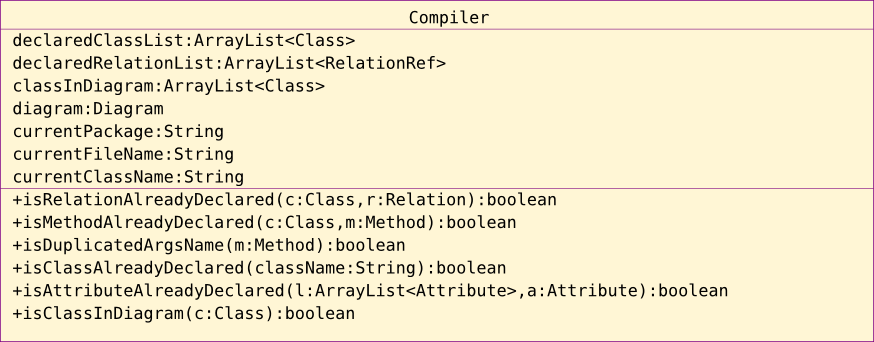
\includegraphics[width=0.9\textwidth]{img/uml_compilatore.png}
  \caption[labelInTOC]{Struttura del codice per l'esecuzione dei controlli semantici.}
\end{center}
\end{figure}

Nel diagramma uml soprastante\footnote{Il digramma è stato creato con cUml2Svg} sono
indicate le strutture dati e le funzioni di supporto per i controlli semantici.
%antonio

\section{Implementazione generatore SVG}

La funzione principale del linguaggio cUml è quella di permettere la creazione 
di diagrammi UML partendo da un modello dati e uno schema di layout.
Come dice il nome del programma il formato prescelto per l'esportazione è SVG
\cite{svg_website:8} ovvero un formato vettoriale creato dal W3C
\cite{w3c_website:9} basato su XML.
La generazione della grafica avviene in due passi principali:
\begin{itemize}
  \item lettura e controllo del modello ad oggetti;
  \item lettura e applicazione dei parametri di layout agli oggetti;
\end{itemize}

Al termine di queste due fasi abbiamo a disposizione una rappresentazione degli
oggetti con i dettagli che permettono il corretto posizionamento all'interno
dello spazio della grafica.
L'unica cosa che rimane da fare a questo punto è la generazione del codice vero
e proprio che costituisce SVG. Per questa fase la scelta dello strumento da
utilizzare è caduta su Apache Velocity \cite{apache_velocity_website:7}, un
motore di 
template parametrico scritto in linguaggio Java che ha permesso di semplificare
di molto il lavoro da compiere.

\subsection{Apache Velocity}
Velocity è uno strumento molto potente e possiede un suo linguaggio interno per
realizzare cicli e controlli condizionali direttamente all'interno del codice
del template, in questo modo è stato semplice creare dei modelli dinamici di
codice che si adattassero allo stato effettivo degli oggetti da disegnare.

\subsection{La gestione dell'esportazione}
Il template è praticamente tutto codice SVG con inclusi controlli condizionali e
cicli per l'adattamento alle condizioni dell'oggetto da disegnare. Per
semplicità e pulizia, il template è stato spezzato in diversi sotto-template che
vengono richiamati ognuno dall'oggetto che ne fa uso.
Nel modello utilizzato da cUml2Svg la struttura è costituita da diversi oggetti:
\begin{itemize}
  \item SVGExporter: è l'oggetto principale che comanda l'esportazione prendendo
  come parametro un Diagramma e i dettagli di esportazione ovvero il nome del
  file da creare e il percorso dove trovare i template di esportazione;
  \item Diagram: come si può intuire è il componente principale del diagramma
  ovvero l'oggetto che contiene tutti i componenti che costituiscono il modello;
  \item Group: rappresenta il blocco logico di esportazione del modello ed è
  quello che raggruppa le classi permettendone la disposizione;
  \item Class: rappresenta l'oggetto vero e proprio, ovvero il componente
  principale del diagramma con attributi e metodi;
  \item Relation: serve per rappresentare le connessioni tra le classi;
\end{itemize}
L'esportazione avviene chiamando il metodo \lstinline{export()} di SVGExporter,
questo provvede a chiamare il metodo \lstinline{render()} del diagramma il quale
ricorsivamente chiama lo stesso metodo di tutti gli oggetti (gruppi e classi)
che si occupano poi di caricare e compilare i template.
Al termine delle chiamate a \lstinline{render()} il controllo ritorna ad
SVGExporter che effettua la scrittura su file del grafico creato.

\subsection{Un esempio di SVG generato}
Il risultato dell'esportazione come detto è SVG, ovvero codice XML che
rappresenta gli oggetti grafici. Quello di seguito è un esempio di codice
generato da uno degli esempi presenti nel capitolo relativo, nello specifico
l'esempio 2.

\begin{lstlisting}[language=xml, caption={Un esempio di codice SVG generato}]
<?xml version="1.0" standalone="no"?>
<!DOCTYPE svg PUBLIC "-//W3C//DTD SVG 1.1//EN" 
  "http://www.w3.org/Graphics/SVG/1.1/DTD/svg11.dtd">
<svg version="1.1"
     width="29.7cm" height="21cm" viewBox="-150 -150 1478 490"
     xmlns="http://www.w3.org/2000/svg">
  <desc>Export of </desc>
  <defs id="definitions">
    <marker
       refX="0"
       refY="0"
       orient="auto"
       style="overflow:visible"
       id="Use">
      <path
         d="M -35.0,11.5 L -0.0,0.0 L -35.0,-11.5 L 
-35.0,11.5 z "
         transform="scale(0.9,0.9)"
         style="fill-rule:evenodd;stroke:#000000;
stroke-width:1pt;marker-start:none"
      />
    </marker>
...
  </defs>
  <g transform="translate(0,0)" >
  <rect
    width="414"
    height="152"
    rx="0"
    ry="0"
    x="0"
    y="0"
    style="fill:#fff6d5;stroke:#800080;stroke-width:1.25;
stroke-miterlimit:4;stroke-dasharray:none"
  />
  <text
    x="20"
    y="38"
    style="font-size:28px;font-style:normal;font-weight:normal;
text-align:start;text-anchor:start;fill:#000000;fill-opacity:1;
stroke:none;stroke-width:1px;stroke-linecap:butt;
stroke-linejoin:miter;stroke-opacity:1;
font-family:Bitstream Vera Sans Mono">
    <tspan
      x="227"
      y="38"
      style="font-size:28px;text-align:center;
text-anchor:middle;font-family:Bitstream Vera Sans Mono">
      org.example.Classe1
     </tspan>
  </text>
  <path
    d="M 0,48 L 414,48"
    style="fill:none;fill-rule:evenodd;stroke:#800080;
stroke-width:1px;stroke-linecap:butt;stroke-linejoin:miter;
stroke-opacity:1"
  />
  <text
    x="20"
    y="76"
    style="font-size:28px;font-style:normal;font-weight:normal;
text-align:start;text-anchor:start;fill:#000000;fill-opacity:1;
stroke:none;stroke-width:1px;stroke-linecap:butt;
stroke-linejoin:miter;stroke-opacity:1;
font-family:Bitstream Vera Sans Mono">
      +x:int=0
  </text>
  <path
         d="M 0,86 L 414,86"
     style="fill:none;fill-rule:evenodd;stroke:#800080;
stroke-width:1px;stroke-linecap:butt;
stroke-linejoin:miter;stroke-opacity:1"
  />
  <text
    x="20"
    y="114"
    style="font-size:28px;font-style:normal;font-weight:normal;
text-align:start;text-anchor:start;fill:#000000;fill-opacity:1;
stroke:none;stroke-width:1px;stroke-linecap:butt;
stroke-linejoin:miter;stroke-opacity:1;
font-family:Bitstream Vera Sans Mono">
      +print():void
  </text>
</g>
...
</svg>
\end{lstlisting}

L'esempio è stato accorciato per brevità, comunque è possibile notare 
che tutto il modello viene scomposto e rappresentato in gruppi
(\lstinline{<g></g>}), rettangoli (\lstinline{<rect></rect>}), testo 
(\lstinline{<text><tpath></tpath></text>}) e linee (\lstinline{<path></path>}).
Da questi elementi prende vita il disegno finale del diagramma:

\begin{figure}[htp]
\begin{center}
  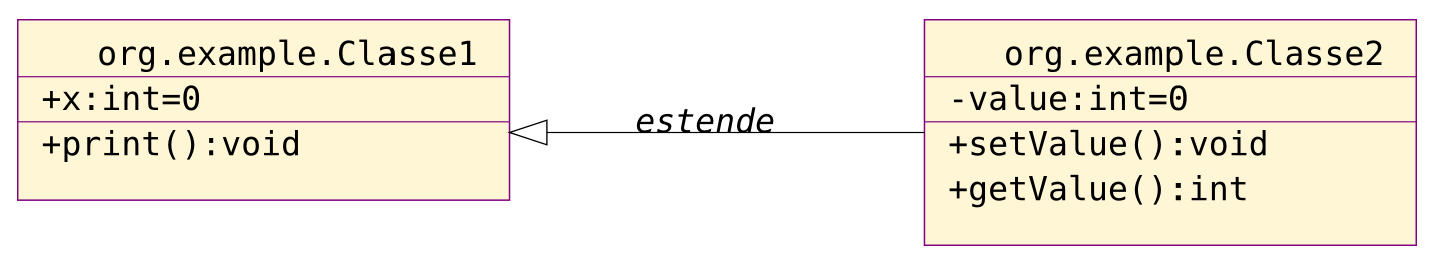
\includegraphics[width=0.9\textwidth]{img/esempio2}
  \caption[labelInTOC]{Risultato dell'esportazione del codice dell'esempio 2}
\end{center}
\end{figure}

%fabio

Per il progetto è stato sviluppato un plugin per Eclipse che si occupa di: \\*
\begin{itemize}
  \item text-highlight
  \item controllo degli errori
  \item compilazione
\end{itemize} 


\subsection{text-hilight}
Il plugin gestisce il \emph{modello dati} e lo \emph{schema di layout} in modi differenti; 
entrambi, infatti, presentano caratteristiche e strutture diverse tra loro.
La classe che esegue la scansione del \emph{modello dati} e ne gestisce l'editor
è la seguente:

\begin{lstlisting}[caption={ModelScanner}, style={java}]
public class ModelScanner extends RuleBasedScanner {
	//TODO controllare tutte le keyword
	private static String[] keywords= { "class","package", "public",
			"private","interface", "methods","extend", "relations", 
			"attributes"  };
	public ModelScanner(ColorManager manager) {
					manager.getColor(ColorConstants.DEFAULT)));
		ArrayList<IRule> rules= new ArrayList<IRule>();	
		Token tokencomment = new Token(new TextAttribute(
						manager.getColor(ColorConstants.COMMENT)));
		//Add rule for processing instructions
		rules.add( new SingleLineRule("//", "\n", tokencomment));
		rules.add( new SingleLineRule("#", "\n", tokencomment));
		rules.add( new MultiLineRule("/*", "*/", tokencomment));
		
		Token token= new Token(new TextAttribute(
				manager.getColor(ColorConstants.KEYWORD), 	//parola
				null, 	//sfondo
				SWT.BOLD));
		WordRule wordRule = new WordRule(new WordDetector());
		for (int i = 0; i < keywords.length; i++) {
			wordRule.addWord(keywords[i], token);
		}		
		rules.add(wordRule);
		
		token = new Token(new TextAttribute(
							manager.getColor(ColorConstants.BRACET)));
		RuleBrace braceRule = new RuleBrace(token);
		rules.add(braceRule);
		
		IRule[] r= new IRule[rules.size()];
		setRules(rules.toArray(r));
	}
}
\end{lstlisting}


Le parole chiave di questo modello sono specificate nella stringa
\emph{Keywords}, inoltre vengono definite le regole per i commenti e viene
utilizzata la classe RuleBrace, che è utilizzata per la gestione delle
parentesi.\\* 
La classe che esegue la scansione dello  \emph{schema di layout} e ne gestisce
l'editor, invece, è la seguente:

\begin{lstlisting}[caption={LayoutScanner}, style={java}]

public class LayoutScanner extends RuleBasedScanner {
	private static String[] keywordslayout= {"@layout","@hide-args",
												"@collapse","@margin"};
	private static String[] keywords= { "class","import","interface"};
	
	public LayoutScanner(ColorManager manager) {
		ArrayList<IRule> rules= new ArrayList<IRule>();
		Token token= new Token(new TextAttribute(
				manager.getColor(ColorConstants.KEYWORD), 	//parola
				null, 																			//sfondo
				SWT.BOLD));
		Token tokenlayout= new Token(new TextAttribute(
				manager.getColor(ColorConstants.LAYOUT), 	//parola
				null, 																		//sfondo
				SWT.BOLD));
		WordRule wordRule = new WordRule(new WordDetector());

		for (int i = 0; i < keywords.length; i++) {
			wordRule.addWord(keywords[i], token);
		}
		for (int i = 0; i < keywordslayout.length; i++) {
			wordRule.addWord(keywordslayout[i], tokenlayout);
		}
		rules.add(wordRule);
		Token tokencomment = new Token(new TextAttribute(
								manager.getColor(ColorConstants.COMMENT)));
		//Add rule for processing instructions		
		rules.add( new SingleLineRule("//", "", tokencomment));
		rules.add( new SingleLineRule("#", "", tokencomment));
		rules.add( new MultiLineRule("/*", "*/", tokencomment));
//gestione colore parentesi
		token = new Token(new TextAttribute(
										manager.getColor(ColorConstants.BRACET)));
		RuleBrace braceRule = new RuleBrace(token);
		rules.add(braceRule);
		IRule[] r= new IRule[rules.size()];
		setRules(rules.toArray(r));
	}
}



\end{lstlisting}



In questo modello le parole chiave sono specificate nella
stringa \emph{Keywords}, mentre le proprietà disponibili sono definite in
\emph{keywordslayout}, in questo modo è possibile gestirle in modo separato.
Per la gestione delle parentesi e dei commenti sono state utilizzate le stesse
tecniche del modello dello \emph{schema di layout}.

\subsection{controllo degli errori} 
Il plugins si occupa di visualizzare, tramite dei marker laterali, gli errori 
commessi in fase di scrittura del \emph{modello dati} e dello \emph{schema di
layout}. \\*
Il controllo degli errori viene eseguito ogni volta che il file su cui si stà lavorando
viene salvato; un esempio del funzionamento è visibile in figura 

\begin{figure}[htp]
\begin{center}
  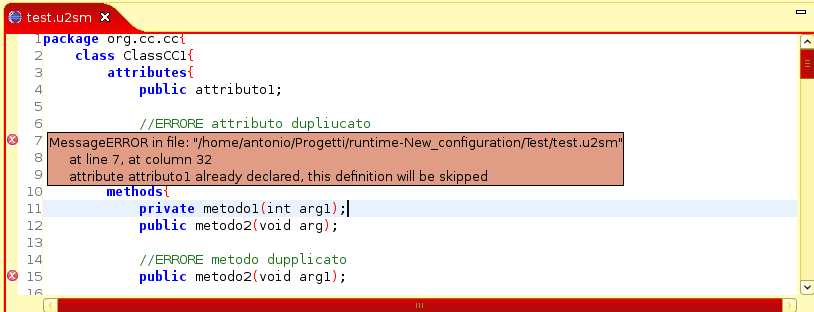
\includegraphics[width=0.9\textwidth]{img/errori_editor.png}
  \caption[labelInTOC]{Gestione degli errori}
\end{center}
\end{figure}

\lstset{escapeinside={(*}{*)}}
\chapter{Esempi d'uso}

In questo capitolo saranno presentati alcuni esempi di utilizzo del linguaggio
cUml sia per la realizzazione del modello dati che per la specifica del layout
di impaginazione.

\section{Esempo di modello dati}
Il modello dei dati è rappresentato all'interno di files con estensione u2sm.

\subsection{Primo esempio semplice}
Il seguente listato definisce una classe di nome Class1 con un attributo
pubblico di tipo intero e con valore iniziale pari a 0. La classe ha inoltre un
metodo pubblico print.
\begin{lstlisting}[caption={Semplice esempio di modello}, style={model}]
package org.example {
  class Classe1 {
    attributes {
      public int x = 0;
    }
  
    methods {
      public void print();
    }
  }
}
\end{lstlisting}

\subsection{Un esempio un po' più complesso}
In questo esempio viene mostrato l'uso delle relazioni tra due classi.

\begin{lstlisting}[caption={Un esempio un po' più complesso}, style={model}]
package org.example {
  class Classe1 {
    attributes {
      public int x = 0;
    }

    methods {
      public void print();
    }
  }

  class Classe2 {
    relations {
      extend org.example.Classe1 ("(1,*)","estende","(1,*)");
    }

    attributes {
      private int value = 0;
    }

    methods {
      public void setValue(int newValue);
      public int getValue();
    }
  }
}
\end{lstlisting}


\section{Esempio di layout}
Quando si è conclusa la realizzazione del modello dati è possibile procedere alla
definizione del layout che indicherà al programma come disporre gli oggetti
all'interno del diagramma SVG.

\subsection{Il primo semplice layout}
In questo esempio viene mostrato come includere il file di modello con gli
oggetti da rappresentare e come includerli nel diagramma in output. Si considera
come input il modello riportato nel listato \ref{model_complex}

\begin{lstlisting}[caption={Un semplice esempio}, style={layout}]
import example(*\ref{model_complex}*).u2sm;
[
  (class org.example.*)
]
\end{lstlisting}

Questo comando indica di includere tutte le classi del package org.example.

\begin{figure}[htp]
\begin{center}
  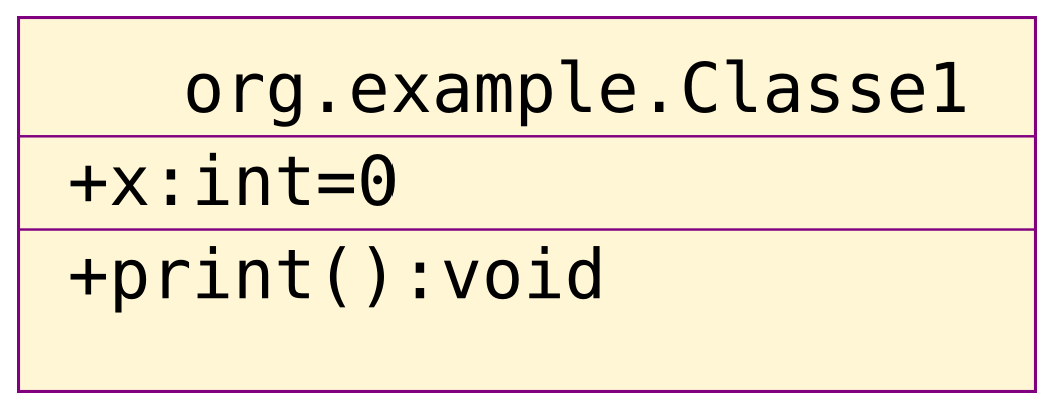
\includegraphics[width=0.5\textwidth]{img/esempio1}
  \caption[labelInTOC]{Risultato dell'esportazione del codice dell'esempio 1}
\end{center}
\end{figure}


\subsection{Un esempio un po' più complesso}
In questo secondo esempio viene mostrato come includere il file di modello con
la definizione degli oggetti e si utilizzano alcuni parametri avanzati come:
\begin{itemize}
\item \lstinline{@hide-args} che permette di nascondere i parametri dei metodi
\item \lstinline{@margin} che permette specificare i margini per un gruppo 
nell'ordine \lstinline{top right bottom left} come da standard W3C.
\end{itemize}

\begin{lstlisting}[language=layout, caption={Un esempio un po' più complesso}, style={layout}, label=layout_simple]
import example(*\ref{model_complex}*).u2sm;
[
  @hide-args
  (class org.example.Classe1)
  [
    @margin 0 0 0 300
    (class org.example.Classe2)
  ]
]
\end{lstlisting}

Ecco il risultato dell'esportazione

\begin{figure}[htp]
\begin{center}
  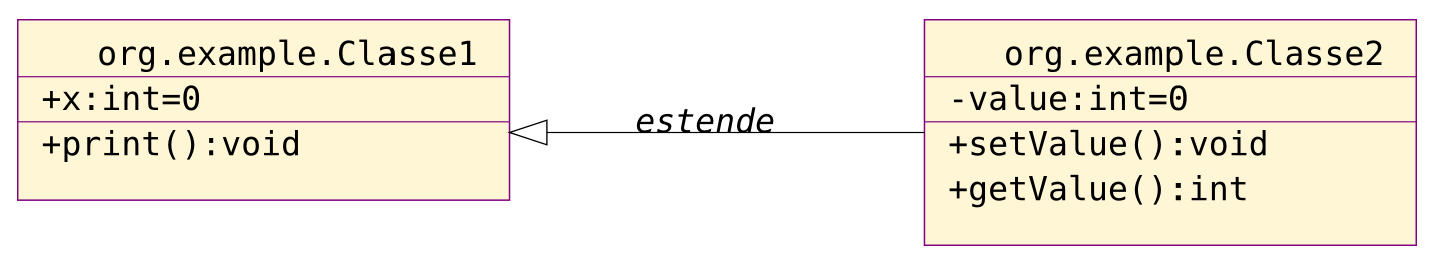
\includegraphics[width=0.9\textwidth]{img/esempio2}
  \caption[labelInTOC]{Risultato dell'esportazione del codice dell'esempio 2}
\end{center}
\end{figure}

\subsection{Il pattern Visitor}

Per dimostrare che il sistemaè utilizzabile anche in un ambito reale, procediamo
ora con l'esempio del pattern Visitor.

\begin{lstlisting}[style={model}, caption={Il modello}]
package visitor{
	class Client{
		relations{
			depend visitor.Visitor("","import","");
			realize visitor.ObjectStructure;
		}
	}
	interface Visitor{
		methods{
			public int VisitConcreteElementA(is ConcreteElementB);
			public VisitConcreteElementB(ConcreteElementB);
		}
	}
	class ConcreteVisitor1{
		relations{
			realize visitor.Visitor;
		}
		methods{
			public VisitConcreteElementA(ConcreteElementA);
			public VisitConcreteElementB(ConcreteElementB);
		}
	}
	class ConcreteVisitor2{
		relations{
			realize visitor.Visitor;
		}
		methods{
			public VisitConcreteElementA(ConcreteElementA);
			public VisitConcreteElementB(ConcreteElementB);
		}
	}
	class ObjectStructure{
		relations{
			depend visitor.Element("","import","");
		}
	}
	class Element{
		methods{
			public Accept(Visitor Visitor);
		}
	}
	class ConcreteElementA{
		relations{
			realize visitor.Element;
		}
		methods{
			public Accept(Visitor Visitor);
			public OperationA();
		}
	}
	class ConcreteElementB{		
		relations{
			realize visitor.Element;
		}
		methods{
			public Accept(Visitor Visitor);			
			public OperationB();
		}
	}
}
\end{lstlisting}

Il layout sfrutta l'alternarsi di disposizione in linea e disposizione in
colonna per allineare glo oggetti nel diagramma.

\begin{lstlisting}[style=layout, caption={Il Layout}]
import visitor.u2sm;
[	
	@layout *x1
	[
		@layout 1x*
		[
			@margin 0 150 0 0
			(class	visitor.Client)
		]
		[
			@layout *x1
			@margin 0 50 0 0
			(interface	visitor.Visitor)
			[
				@layout 1x*
				(class	visitor.ConcreteVisitor1)
				(class	visitor.ConcreteVisitor2)
			]
		]
	]
	[
		@layout 1x*
		@margin 50 0 0 0
		(class	visitor.ObjectStructure)
		[
			@margin 0 0 0 150
			@layout *x1
			(class	visitor.Element)
			[
				@layout 1x*
				(class	visitor.ConcreteElementA)
				(class	visitor.ConcreteElementB)
			]
		]
	]
]
\end{lstlisting}

Ed ora l'output generato.

\begin{figure}[htp]
\begin{center}
  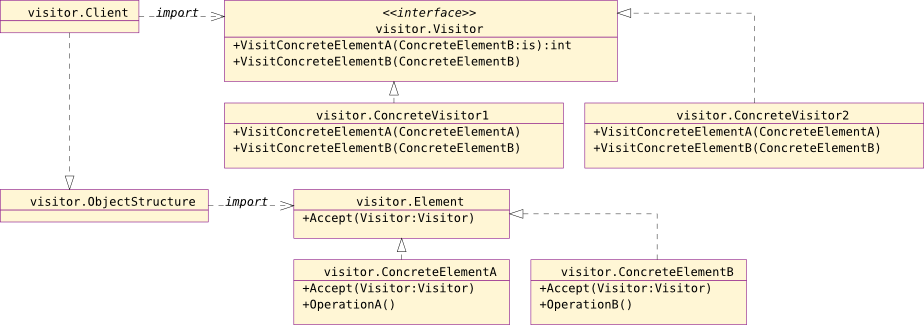
\includegraphics[angle=90,width=0.5\textwidth]{img/visitor}
  \caption[labelInTOC]{Risultato dell'esportazione del codice visitor}
\end{center}
\end{figure}



%luca %antonio %fabio
\chapter{Conclusione}
%fabio


\bibliographystyle{plain}
\bibliography{bibliography.bib}

\end{document}